\documentclass[a4paper,11pt]{article}

% 数式
\usepackage{amsmath,amsfonts,hyperref,amssymb,empheq}
\usepackage{latexsym,mathtools,array}
\usepackage{physics}
\usepackage{bm}
% 画像
\usepackage[dvipdfmx]{graphicx}

\makeatletter % some generic helpers
\newcommand{\LCASES}[1]{$\m@th\displaystyle{#1}$\hfil}
\newcommand{\CCASES}[1]{\hfil$\m@th\displaystyle{#1}$\hfil}
\newcommand{\RCASES}[1]{\hfil$\m@th\displaystyle{#1}$}
\makeatother
\newcases{ecases}{\quad}{\CCASES{##}}{\LCASES{##}}{\lbrace}{.}
\newcases{ecases*}{\quad}{\CCASES{##}}{{##}\hfil}{\lbrace}{.}

\begin{document}

\title{関数マップの拡張可能性について}
\author{Yoshinori Watanabe \\ \href{mailto::ywatanabe750@fuji.waseda.jp}{ywatanabe750@fuji.waseda.jp}}
\date{\today}
\maketitle

\begin{abstract}
関数マップの拡張例としては
\begin{itemize}
    \item ε演算の変更 例えば$f'=af(f(x/a))$のような積の形を用いる
    \item x(関数の定義域、値域)を1次元から高次元に拡張
    \item 一回で複数の関数適用$\cdot$を行う
    \item 多値関数、確率分布に値を持つ関数(確率過程)への拡張
    \item 定義域、値域の空間の変更(多次元トーラスなど)
\end{itemize}
などが考えられる。このようなあり得る拡張を包括するような概念、手法を考えたい。
\end{abstract} 
    
\section{機械学習からの視点}
Attentionに見られるfを行列積$f=W_f X$として(Transformerの記法では$Q=W_qX, K=$)表現する方法は中間の次元Mが可変で行列Wは可変でありかつ学習によって変化しうるという点が特徴的である。

非線形な関数とそれらの間の関数を高次元空間での線形関数とそれらの間の内積に変換する方法は機械学習においてはカーネル法と呼ばれ、よく用いられている。
これは中間の次元を大きくする方法であるが、それとは別に実用的にはx(入力の次元)を多次元にしたと言えるMulti Head Attention(MHA)が高性能に重要であることが知られている。各次元の関数マップを"混ぜ合わせる"操作をMulti Head Attentionの後段のMLP(Multi-Layer Perceptron)が行っているとみなせる。$W_q$などのAttention,MLPの行列は学習によって決定されるものだが、力学系として混ぜ合わせの性質を見ることができる。

行列Wが学習によって変化するというのは自然言語や画像からの情報を取捨し、そこから推論を行うのに必要な機能だが、Attentionを力学系としてみたときの性質を見るには複雑すぎる。
\cite{PhysRevLett.94.058102} ではMLPが連続することで学習結果の境界が複雑化し、層を経るごとにカオス的な挙動になることが示されている。MLPとAttentionを交互に行うことで軌道を安定化させている可能性がある。
そもそもDNNが長らく実用化されなかったのは学習過程において層を経るごとに勾配が消失する問題と過学習の問題のためだとも言われている。Magic Numberの研究はそれとは違ったカオス的性質を持ちうるといういみでDepp MLPが問題をはらんでいると主張している。\cite{kobayashi2024analyzing}では逆にMLPとAttentionの役割分担としてAttentionが混ぜ合わせ、MLPが知識の付加を担っているとしている。

一方でAttentionにおけるVの位置づけの関数マップにおける対応は単純ではない。既知の線形補間型関数マップ$f'=()f+~$が可算、あるいは線形補間を用いて書かれるのに対し、(Self,Mutual)Attentionは$A=QK$(の各要素をsoftmax化したもの)とVの行列乗算$softmax(QK^T)/\sqrt{d}V$で書かれる。線形に近い場合は$softmax(QK^T)V\simeq\epsilon QK^TV:=QE'=Q(I+E)=Q+QE=:Q+\epsilon K^TV$
とQをf, $K^TV$を$f\cdot f$とみなすと線形補間関数マップに近い形で書かれる。$K^TV=E'=I+E$が単位行列に近いという仮定を置いた。softmaxを線形とみなしKVのまとまりを近似する方法(Linear Attenion)はカーネル法や計算の高速化、データ圧縮とも関連して理論、応用の観点から盛んに研究されている\cite{katharopoulos2020transformersrnnsfastautoregressive}。

\begin{figure}[htbp]
\begin{center}
\includegraphics[width=200pt]{fig/summary.png}
\caption{Attentionの構成図}
\end{center}
\end{figure}

\begin{figure}[htbp]
\begin{center}
\includegraphics[width=200pt]{fig/MHA.png}
\caption{Multi Head Attentionの構成図}
\end{center}
\end{figure}
  
\begin{figure}[htbp]
\begin{center}
\includegraphics[width=200pt]{fig/Transformer.png}
\caption{Multi Head Attention, MLPを使ったTransformerの構成図}
\end{center}
\end{figure}
  
\section{数学、圏論からの視点}
一般には関数マップは関数の集合$\cal{F}=\{f_1,f_2,...,g_1,g_2,..\}$に対する演算と言える。通常数学では群(加減算のみ)、環(加減乗算)、体(加減乗除)の演算に対して閉じている系が考えられることが多く、関数適用演算子$\cdot$のようなさらに多くの演算を加えた場合については余り考えられれていない。圏論では異なる(あるいは同一の)群や環の間の(準)同型写像を一般化した関手とそれらの間の写像である自然変換などが研究対象となっている。

ベクトル空間としての構造を持つxとそれに対する写像に対する写像を組み合わせたAttention mapの構造は圏論で記述できる。一方可算に対する準同型性$T(F(x,y))=F(T(x))+F(T(y))$を持った関数マップはパラメーターεの変化とみなすことができる。

関数fを射、fの定義域、値域の値xを対象、関数マップを関手とした圏とfを対象、fに対する関数マップを射、異なるεを持つ関数マップ(射)を移す関手としてみた圏が考えられる。圏論によればこの2つの圏の間には自然変換$\eta:C \rightarrow D, a \mapsto F(a)$がありさらに米田の補題によれば対象xに対して対象を射に、射を射の射に移すような関手$H^x$と任意の関手に対する自然変換の集合$Nat(H^x,F)$に対し$Nat(H^x,F) \simeq F(x)$が成り立つとされる。
しかしこの関係、補題が成り立つには関数マップが線形補間の形である他に定義域、値域が同じであるという制約が課されることになる。

\begin{figure}[htbp]
\begin{center}
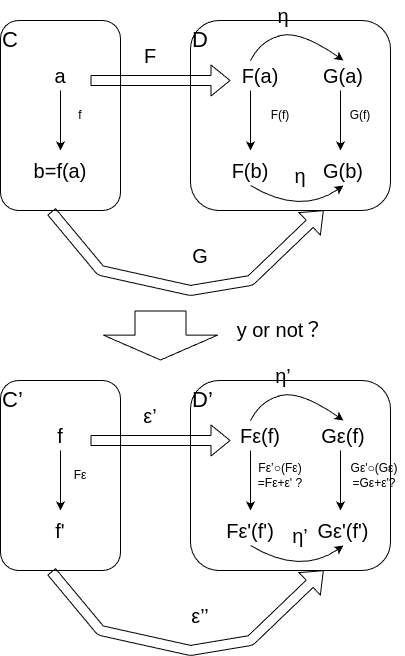
\includegraphics[width=200pt]{fig/yoneda.png}
\caption{関手としての関数マップと自然変換η,yは米田写像かもしれない}
\end{center}
\end{figure}
  
関手、自然変換の存在は準同型であれば変換の性質は問わないため要素xの属する空間、演算の種類を一般化することができる。最も簡単な例は線形補間関数マップのeの方に載せた形であり$e^f$を$f$に置き換えてを$f=f^(1-\epsilon)f*(f\cdot f)^\epsilon$と積で書かれ、定義域、値域は正の値のみになる。同様に円や複素数からリーマン球面への変換などが考えられる。
関数マップの上位の存在とも言える空間や演算の変換自体も自然変換で表されるというのが米田の補題の主張と言えるかもしれない(言えると非自明かもしれない)。

Attentionでは$f\cdot f$相当の行列積$QK^T$はと線形変換Q($R^n \rightarrow R^m$)と共役な線形変換K($R^m \rightarrow R^n$)に分解された。これを圏論的に捉えると随伴という関係にあると言え、xと$W_qx$等同じ処理を異なる表現で行っているといえる。

\section{一般化}
上記の見方から一般化の方向性を整理すると
\begin{itemize}
  \item Q,Kの行列次元の拡大
  \item MLP以外の要素(CNNなど)をAttentionに挟む
  \item 準同型性を持った演算、空間への一般化
  \item 関数マップ(可算)とAttention(行列積)の不一致を埋める
\end{itemize}
といったものが考えられる。

要素(context)xの定義域として関数空間を取ることもできるがカーネル法の基礎となっているリースの表現定理によってヒルベルト空間の元、計算機上では有限次元ベクトル空間で近似されるそれに制限される。

TransformerがMulti Head AttentionとMLPを交互に挟んだ形であるのは先行研究\cite{Inoue_2022}と関連して限られた計算資源の中で安定した生成結果を生む理由を力学系の観点から説明できるかもしれない。MLPの連続が不安定であるようにAttentionの連続が並列多次元の要素が混ざり合わない以外のよくない性質を持っていると主張できないだろうか。MLPを固定的な並べ替えに入れ替えることで実験できそうである。

線形補間型関数マップの準同型性、generated mapができる性質に着目し、拡張するなら準同型な演算がありさえすればいいのでxの定義域、値域が有限体や楕円曲線などの代数曲線上であり、その上での演算であってもいい。しかし有限要素に対する畳み込み演算は潰れてしまうのであまり面白くない。連続値のxの定義域、値域のトポロジカルな性質がfの固定点の数や周期軌道に影響を与える性質はありそうである。
関数適用$\cdot$を関手とみなした場合は極限をとることができるようである。

関数マップ(可算)とAttention(行列積)の不一致を埋めるのが最も未解明の部分が多いように思われる。関数マップの$\epsilon$,Attentionのsoftmaxの傾きが小さい極限においても
一致しないことがTransformerが高階関数を処理できるという主張の厳密な理解を妨げている。

\subsection{批判}
以上の論考で関数マップやTransformer、LLMの新しい性質を導き出せたわけではない。かろうじてAttentionを使ったアーキテクチャの限界を示氏うる可能性があると言えるかもしれない。
\cite{Inoue_2022}で具体的に示されたようにLUT(Look Up Table)として表現された関数の軌道の様々な空間での性質(固定点、周期、カオスといった分類は成り立つのか、ヒルベルト空間の元に対しては成り立つが無限に折り畳まれた関数はその元となりうるのか?)とその自然言語、画像処理における意味付けは非常に興味深い研究対象のように思える。

\bibliographystyle{jplain}
\bibliography{fmapextend_ref}
\end{document}
